%"###############################################
%
% Profils post opératoires
%
%###############################################

% RTUPB
%
%###############################################

\begin{figure}[H]
\centering
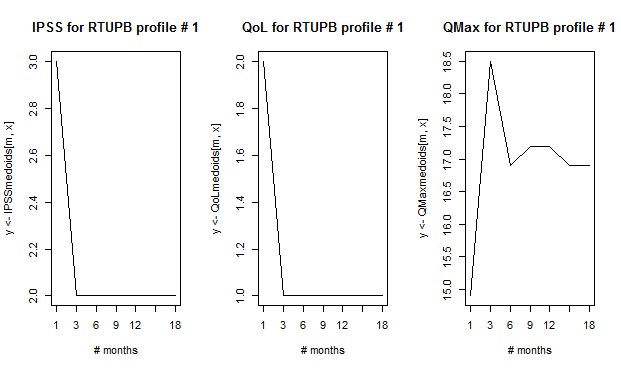
\includegraphics[width=0.75\textwidth]{../Fig/RTUPB/rtupb-profil-post-01.png}
\caption{RTUPB: profil de guérison 1/13}
\end{figure}

Le profil des patients, ci-dessus, montre un bénéfice rapide de l'opération, dès 3 mois, avec une qualité de miction (Qmax) qui progresse spectaculairement à 3 mois, et se stabilise à un régime de croisière à partir de 6 mois (~17.0 ml/s).

\begin{figure}[H]
\centering
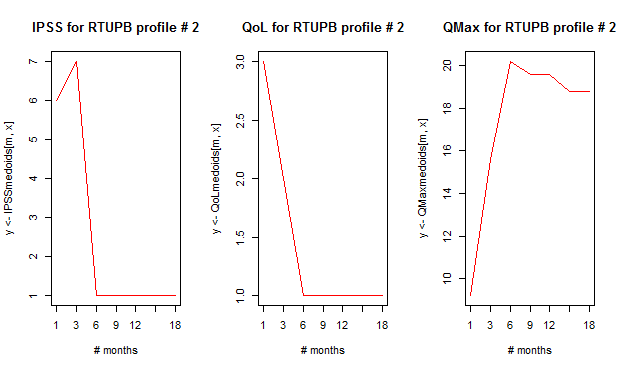
\includegraphics[width=0.75\textwidth]{../Fig/RTUPB/rtupb-profil-post-02.png}
\caption{RTUPB: profil de guérison 2/13}
\end{figure}

Le profil des patients, ci-dessus, montre un bénéfice progressif de l'opération, et stable à partir de 6 mois. La qualité de miction (Qmax) se stabilise à partir de 6 mois entre 18 et 20 ml/s.

\begin{figure}[H]
\centering
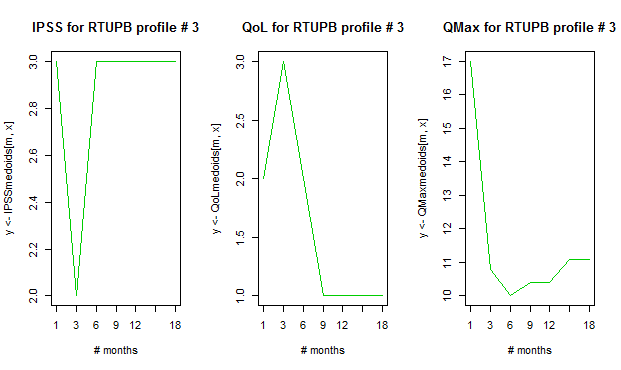
\includegraphics[width=0.75\textwidth]{../Fig/RTUPB/rtupb-profil-post-03.png}
\caption{RTUPB: profil de guérison 3/13}
\end{figure}

Le profil des patients, ci-dessus, montre un ressenti négatif à 3 mois (pic en hausse de QoL, pic en baisse de IPSS), et une dégradation significative de la qualité de miction (Qmax). L'indication QoL par contre redescend à partir de 9 mois. Peut-on parler médicalement d'un résultat décevant de l'opération ?

\begin{figure}[H]
\centering
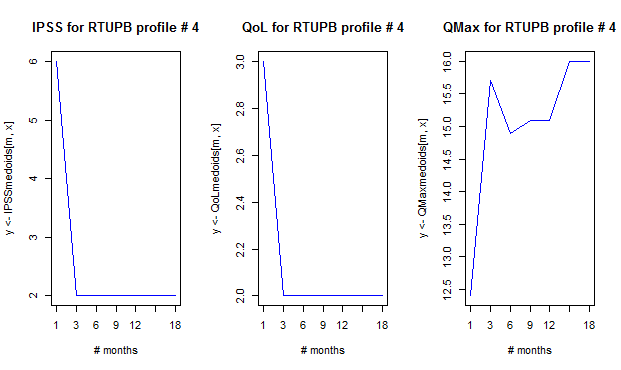
\includegraphics[width=0.75\textwidth]{../Fig/RTUPB/rtupb-profil-post-04.png}
\caption{RTUPB: profil de guérison 4/13}
\end{figure}

Le profil des patients, ci-dessus, est globalement assez proche de celui de la première classe, avec une évolution différente de la qualité de miction (Qmax) avec des valeurs inférieures tout au long du suivi post-opératoire.

\begin{figure}[H]
\centering
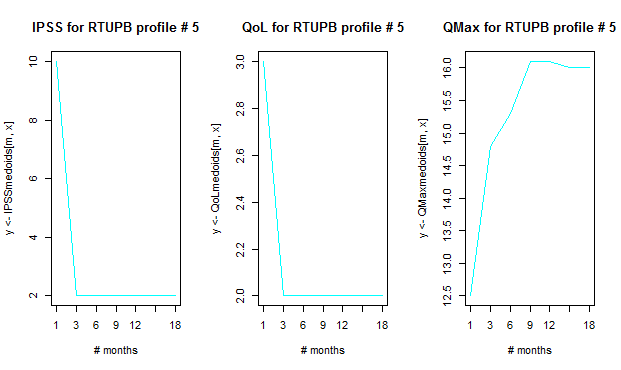
\includegraphics[width=0.75\textwidth]{../Fig/RTUPB/rtupb-profil-post-05.png}
\caption{RTUPB: profil de guérison 5/13}
\end{figure}

Ici aussi, le profil des patients ci-dessus, est assez proche de celui de la première classe, avec une évolution différente de la qualité de miction (Qmax) plus progressive et sans pic à 3 mois.

\begin{figure}[H]
\centering
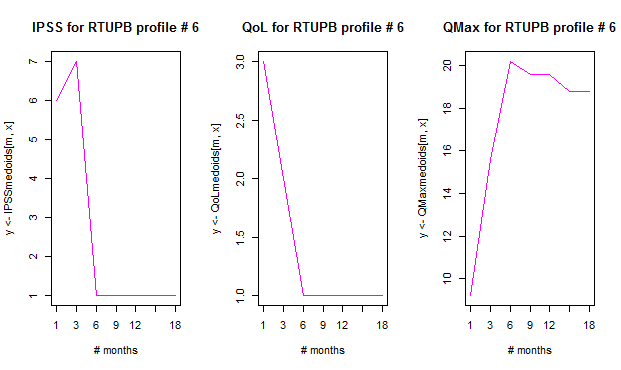
\includegraphics[width=0.75\textwidth]{../Fig/RTUPB/rtupb-profil-post-06.png}
\caption{RTUPB: profil de guérison 6/13}
\end{figure}

Le profil des patients, ci-dessus, est globalement très proche de celui de la deuxième classe, avec des effets post-opératoires bénéfiques à partir de 6 mois.

\begin{figure}[H]
\centering
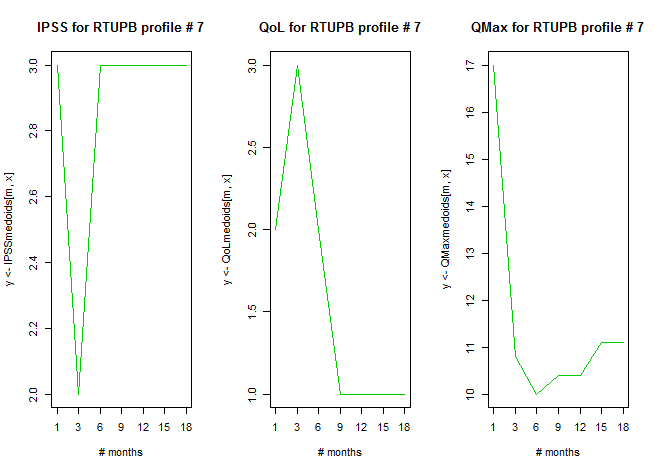
\includegraphics[width=0.75\textwidth]{../Fig/RTUPB/rtupb-profil-post-07.png}
\caption{RTUPB: profil de guérison 7/13}
\end{figure}

Le profil des patients, ci-dessus, est globalement très proche de celui de la troisième classe, avec des résultats décevants.

\begin{figure}[H]
\centering
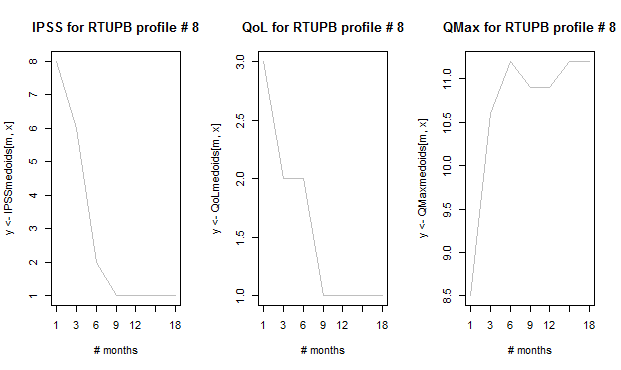
\includegraphics[width=0.75\textwidth]{../Fig/RTUPB/rtupb-profil-post-08.png}
\caption{RTUPB: profil de guérison 8/13}
\end{figure}

Le profil des patients, ci-dessus, montre un bénéfice de l'opération étalé sur les 9 premiers mois. La qualité de miction (Qmax) se stabilise à partir de 6 mois (~11 ml/s).

\begin{figure}[H]
\centering
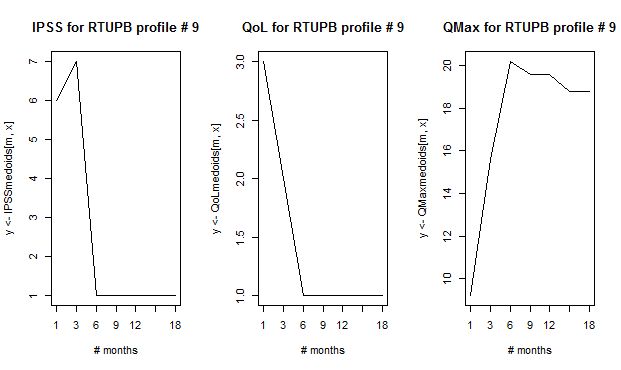
\includegraphics[width=0.75\textwidth]{../Fig/RTUPB/rtupb-profil-post-09.png}
\caption{RTUPB: profil de guérison 9/13}

\end{figure}

Le profil des patients, ci-dessus, est globalement très proche de celui de la deuxième classe, avec des effets post-opératoires bénéfiques à partir de 6 mois.

\begin{figure}[H]
\centering
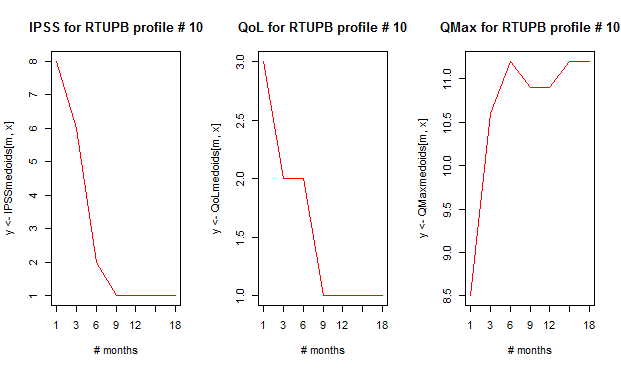
\includegraphics[width=0.75\textwidth]{../Fig/RTUPB/rtupb-profil-post-10.png}
\caption{RTUPB: profil de guérison 10/13}
\end{figure}

Le profil des patients, ci-dessus, très proche de celui de la huitième classe, montre un bénéfice de l'opération étalé sur les 9 premiers mois. La qualité de miction (Qmax) se stabilise à partir de 6 mois (~11 ml/s).

\begin{figure}[H]
\centering
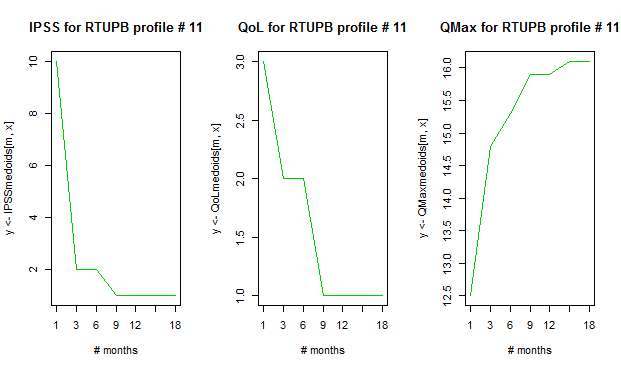
\includegraphics[width=0.75\textwidth]{../Fig/RTUPB/rtupb-profil-post-11.png}
\caption{RTUPB: profil de guérison 11/13}
\end{figure}

Le profil des patients, ci-dessus, assez proche de celui de la huitième classe, montre un bénéfice de l'opération étalé sur les 9 premiers mois. La qualité de miction (Qmax) est au départ meilleure et se stabilise plus lentement après un an (~11 ml/s).

\begin{figure}[H]
\centering
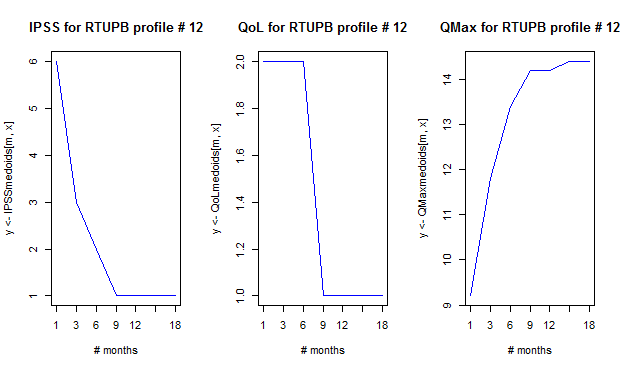
\includegraphics[width=0.75\textwidth]{../Fig/RTUPB/rtupb-profil-post-12.png}
\caption{RTUPB: profil de guérison 12/13}
\end{figure}

Le profil des patients, ci-dessus, assez proche de celui de la huitième classe, montre un bénéfice de l'opération étalé sur les 9 premiers mois, avec une QoL qui ne descend qu'après 6 mois et une qualité de miction (Qmax) qui se stabilise plus lentement après un an (~14 ml/s).

\begin{figure}[H]
\centering
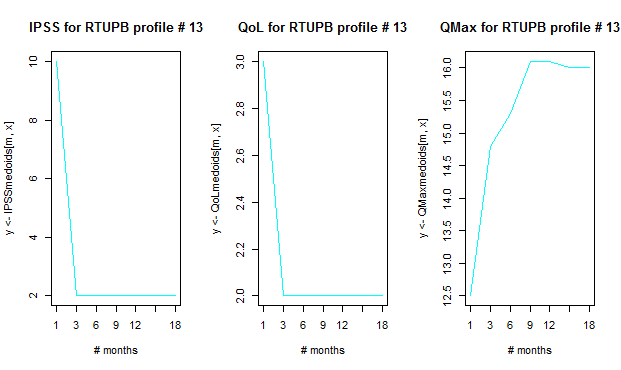
\includegraphics[width=0.75\textwidth]{../Fig/RTUPB/rtupb-profil-post-13.png}
\caption{RTUPB: profil de guérison 13/13}
\end{figure}

Le profil des patients, ci-dessus, est globalement assez proche de celui de la première classe, avec une évolution différente de la qualité de miction (Qmax) avec des valeurs inférieures tout au long du suivi post-opératoire.

En résumé, il semblerait donc que d'un point de vue dynamique des profils de guérison, les 13 classes initiales se factorisent en 4 classes:
\begin{itemize}
\item résultat post-opératoire positif à partir de 3 mois (4 des 13 classes initiales)
\item résultat post-opératoire positif à partir de 6 mois (3 des 13 classes initiales)
\item résultat post-opératoire positif à partir de 9 mois (4 des 13 classes initiales)
\item résultat post-opératoire décevant à partir de 3 mois (2 des 13 classes initiales)
\end{itemize}

% VPPBS
%
%###############################################

\begin{figure}[H]
\centering
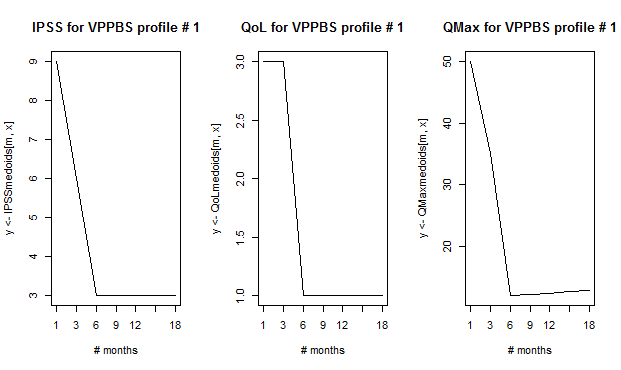
\includegraphics[width=0.75\textwidth]{../Fig/VPPBS/vppbs-profil-post-01.png}
\caption{VPPBS: profil de guérison 1/12}
\end{figure}

\begin{figure}[H]
\centering
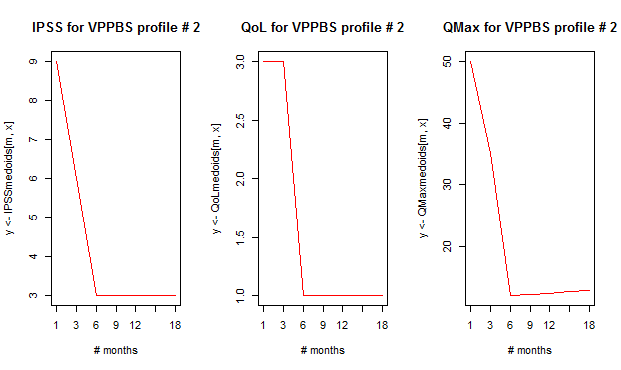
\includegraphics[width=0.75\textwidth]{../Fig/VPPBS/vppbs-profil-post-02.png}
\caption{VPPBS: profil de guérison 2/12}
\end{figure}

\begin{figure}[H]
\centering
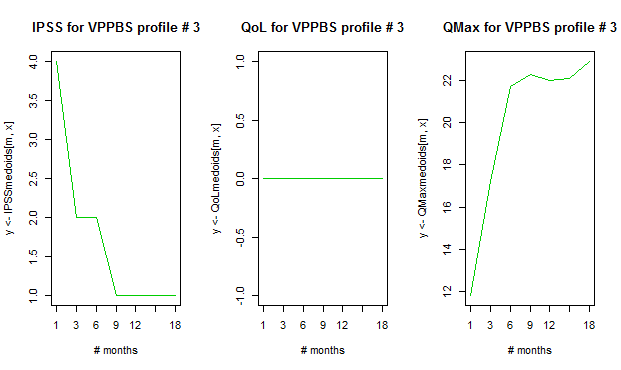
\includegraphics[width=0.75\textwidth]{../Fig/VPPBS/vppbs-profil-post-03.png}
\caption{VPPBS: profil de guérison 3/12}
\end{figure}

\begin{figure}[H]
\centering
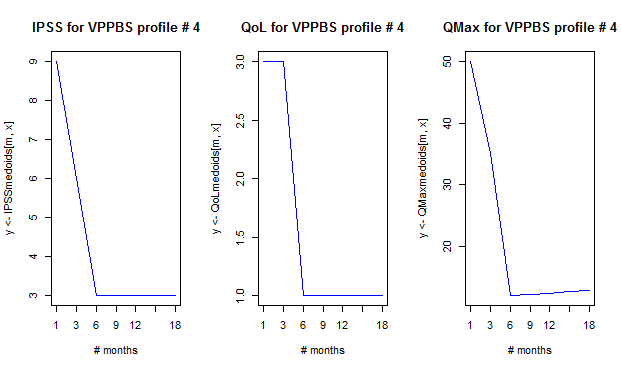
\includegraphics[width=0.75\textwidth]{../Fig/VPPBS/vppbs-profil-post-04.png}
\caption{VPPBS: profil de guérison 4/12}
\end{figure}

\begin{figure}[H]
\centering
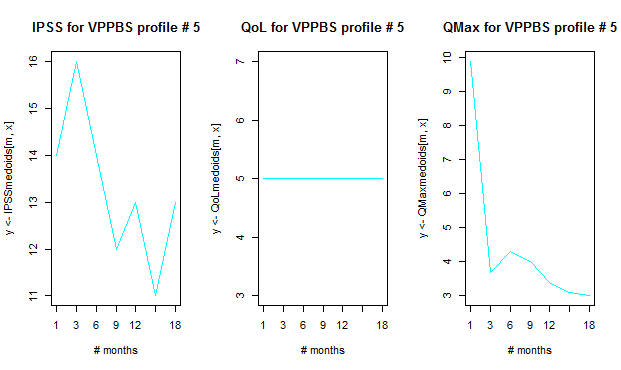
\includegraphics[width=0.75\textwidth]{../Fig/VPPBS/vppbs-profil-post-05.png}
\caption{VPPBS: profil de guérison 5/12}
\end{figure}

\begin{figure}[H]
\centering
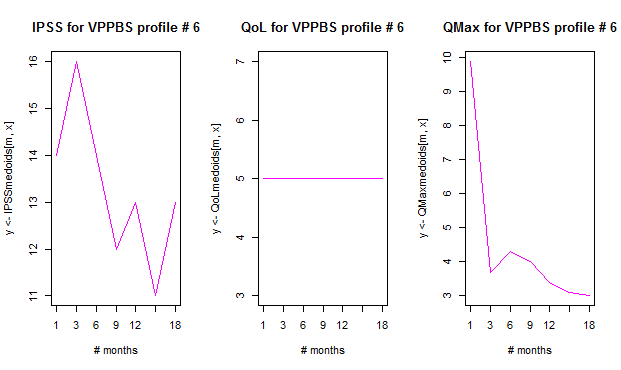
\includegraphics[width=0.75\textwidth]{../Fig/VPPBS/vppbs-profil-post-06.png}
\caption{VPPBS: profil de guérison 6/12}
\end{figure}

\begin{figure}[H]
\centering
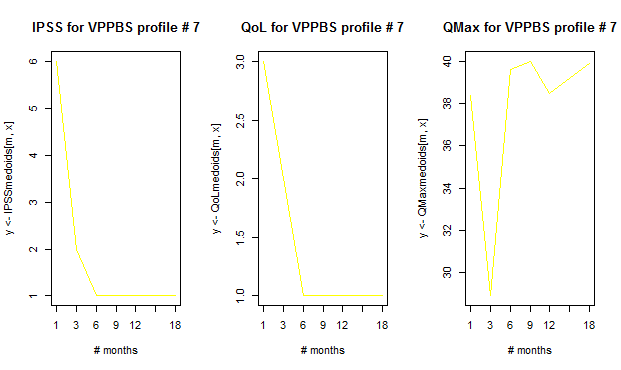
\includegraphics[width=0.75\textwidth]{../Fig/VPPBS/vppbs-profil-post-07.png}
\caption{VPPBS: profil de guérison 7/12}
\end{figure}

\begin{figure}[H]
\centering
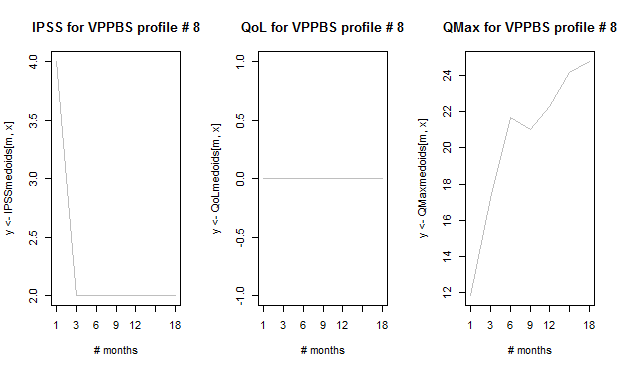
\includegraphics[width=0.75\textwidth]{../Fig/VPPBS/vppbs-profil-post-08.png}
\caption{VPPBS: profil de guérison 8/12}
\end{figure}

\begin{figure}[H]
\centering
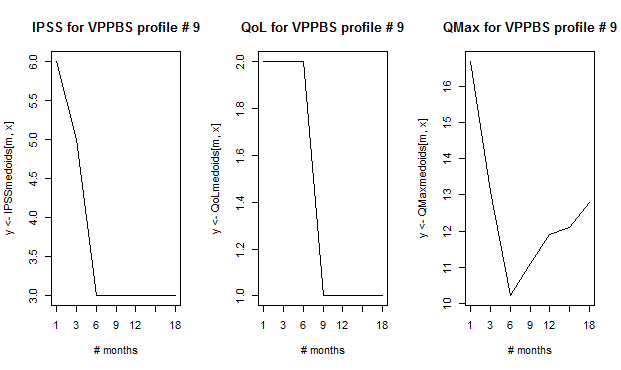
\includegraphics[width=0.75\textwidth]{../Fig/VPPBS/vppbs-profil-post-09.png}
\caption{VPPBS: profil de guérison 9/12}

\end{figure}

\begin{figure}[H]
\centering
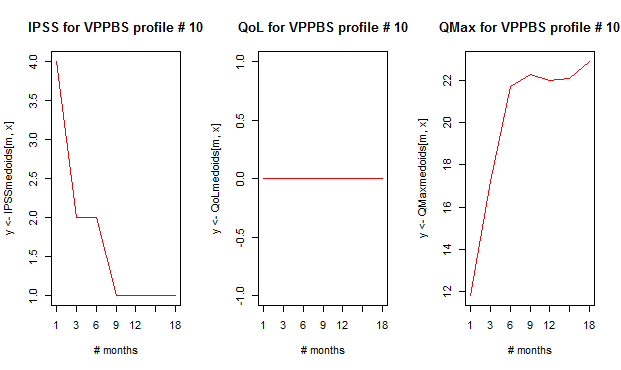
\includegraphics[width=0.75\textwidth]{../Fig/VPPBS/vppbs-profil-post-10.png}
\caption{VPPBS: profil de guérison 10/12}
\end{figure}


\begin{figure}[H]
\centering
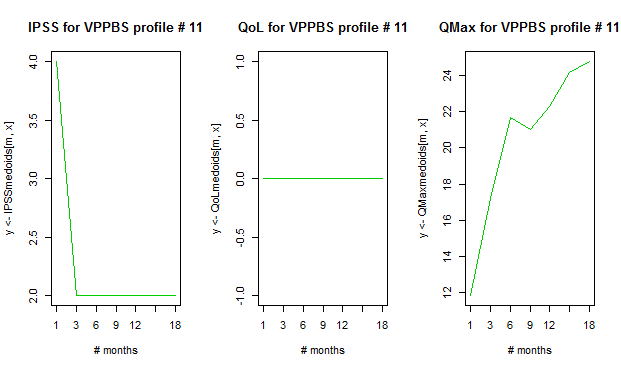
\includegraphics[width=0.75\textwidth]{../Fig/VPPBS/vppbs-profil-post-11.png}
\caption{VPPBS: profil de guérison 11/12}
\end{figure}

\begin{figure}[H]
\centering
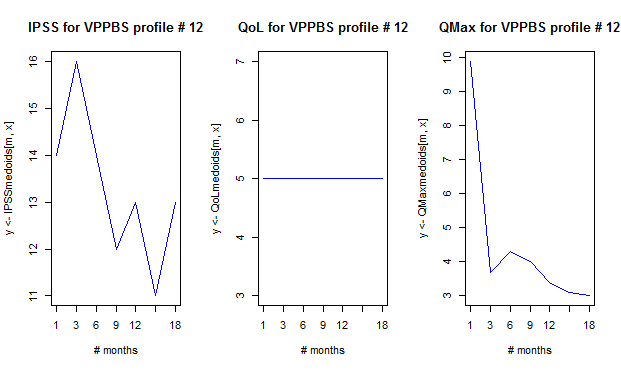
\includegraphics[width=0.75\textwidth]{../Fig/VPPBS/vppbs-profil-post-12.png}
\caption{VPPBS: profil de guérison 12/12}
\end{figure}


%
%##########################
%# CONCLUSION
%##########################